\documentclass{article}
\usepackage[colorlinks]{hyperref}
\usepackage[printonlyused,withpage]{acronym}
\usepackage{float}
\usepackage{natbib}
\usepackage{graphicx}
\author{Christopher Bainbridge}
\title{Underwater Optical Wireless Communications - A Background}

\begin{document}
\maketitle

\begin{abstract}
This document serves as a background and brief summary of \ac{UOWC}. It describes information required for the project, a description of current systems (both research and commercial) as well as the developed system at \ac{KAUST}. It then proceeds to suggest solutions to overcome current issues.
\end{abstract}

\section{Introduction}
There are three main types of communicating wirelessly underwater - acoustic, RF and optical. Acoustic transmissions are characterized by long range but low data rates. RF transmissions are characterized by high throughput but only at very short distances. Optical transmissions sit halfway between these, allowing high throughput at medium ranges, but at the expense of being affected by the environment of the wireless channel.

\section{General Background}
This section summarizes a general background in \ac{UOWC} systems.

\subsection{Light Propagation in Water}
This section lists with short descriptions the issues \ac{UOWC} communications face underwater.

\subsubsection{Absorption and Scattering}
A small fraction of light will be absorbed, and another part scattered, by the water. This becomes more prevalent as the water type degrades, thus propagation is far more challenging.

\subsubsection{Turbulence}
The refraction index can vary along the propagation path due to fluctuations in the density, salinity and temperature of the underwater environment. This is known as scintillation and will degrade performance.

\subsubsection{Pointing and Alignment}
Optical beams are very narrow and thus LOS must be maintained for reliable link performance. Tracking is required between nodes to maintain this.

\subsubsection{Background Noise}
As the visible spectrum of light is being used, noise from other light sources including the Sun can have an effect. In general, deep ocean is less noisy than harbor side.

\subsubsection{Multipath interference and dispersion}
Multipath interference is produced when an optical signal reaches the detector after encountering multiple scattering objects or reflections from other underwater bodies. The signal can be time dispersed thus decreasing the symbol rate due to \ac{ISI}. It is very dependent on the operating conditions, and has been concluded that this effect is only really present in highly turbid environments. Spatial diversity may help to reduce the effects of multipath interference.

\subsubsection{Physical obstructions}
Anything that might get in the way such as marine animals will cause momentary loss of signal at the receiver. The light will also attract marine animals, especially at depth. Error correction, signal processing techniques and redundancy measures are required to ensure re-transmission of data when lost.



\subsection{Water Types}
The literature classifies water types in \ac{UOWC} into these main classes.

\subsubsection{Pure Water and Pure Sea Water}
Pure water is the cleanest water type and has no suspended particulate matter. Pure sea water is pure water but with the addition of salts, although this is assumed to be negligible in visible spectrum, thus making pure sea water and pure water equivalent.

\subsubsection{Coastal Ocean}
Coastal ocean displays more severe absorption and scattering due to the increased concentration of dissolved particles.

\subsubsection{Turbid Harbor}
This is the most hostile environment for optical communications, with the highest concentration of suspended and dissolved particles leading to increased absorption and scattering.




\subsection{Configurations of UOWC}
There are 4 types of link configurations with regards to \ac{UOWC}.

\subsubsection{Point to Point \ac{LOS}}
This is the most typical configuration. Both nodes employ the same transceiver and light sources. Typically the beam angles are narrow, thus requiring precise pointing between nodes.

\subsubsection{Diffused \ac{LOS}}
A point to point link with a large divergence angle allows a signal to be 'broadcast' from one node to multiple remote nodes. Attenuation will be large though due to the increased interaction area with the water. This is useful only if short communication distances and lower data rates are required.

\subsubsection{Retro-reflector \ac{LOS}}

Instead of having both ends transmit a signal, the remote node reflects back the received light whilst encoding its response on it. This is ideal for nodes with low power and weight requirements, but the signal will degrade significantly due to backscatter and additional attenuation through the water.

\subsubsection{\ac{NLOS}}
The signal can be 'bounced' off the sea surface, allowing transmissions to propagate further if there are underwater obstacles present. Of course, the light will be reflected in a somewhat random way depending on wind or other turbulence sources, causing signal dispersion and degradation.


\section{System design}
A generic \ac{UOWC} system incorporates a source generating information to be transmitted, a transmission modulator onto the optical carrier, a transmitter equipped with projection optics and beam steering elements to focus and steer the beam, a detector converting optical to electrical signals and then a subsequent signal processing unit and demodulator.

\subsection{Transmitter}
The transmitter normally uses the blue-green portion of the spectrum. Output power can range from 10 mW to 10 W. Lasers or \ac{LED}s can be used. Lasers have faster switching time (meaning higher data rates can be supported as the modulation bandwidth higher) and higher optical power (meaning higher range), but \ac{LED}s are cheaper, simpler, less temperature dependent and more reliable. Lasers have a much smaller viewing angle than \ac{LED}s.

\subsection{Receiver}
The receiver should have a wide \ac{FOV}, high gain and provide high \ac{SNR}. They are photo sensors that come in a range of types.

According to the literature, currently semiconductor photo-sensors (mainly \ac{PIN} photodiodes) are the best fit for \ac{UOWC}.

\subsubsection{\ac{APD}}
A highly sensitive semiconductor that exploits the photoelectric effect to convert light to electricity.

*** This is from first-sensor.com *** \\
As in the case of standard diodes, photons generate electron-hole pairs, which are accelerated by the applied external voltage such that further electrons are introduced to the conduction band by means of impact ionization. These secondary electrons can in turn absorb sufficient energy to raise further electrons into the conduction band. A multiplication factor of several hundred can thus be achieved.

Avalanche diodes are usually employed in the case of very low optical signal strengths, but are also used for applications with high modulation frequencies. As of frequencies of approx. 60 MHz, the noise level heightened by the avalanche effect is generally lower than that produced by a conventional diode in combination with external electronic amplification.

\subsubsection{\ac{SPAD}}
*** This is from Wikipedia ***\\
A solid-state photodetector in which a photon-generated carrier (via the internal photoelectric effect) can trigger a short-duration but relatively large avalanche current.

The fundamental difference between SPADs and APDs is that SPADs are specifically designed to operate with a reverse-bias voltage well above the breakdown voltage. This kind of operation is also called Geiger-mode in the literature (as opposed to the linear-mode for the case of an APD).

\subsubsection{\ac{PMT}}
A vacuum tube which is very sensitive to light. They have high gain, low noise, a high frequency response and a large collection area, but they are also large, have higher power consumption and are quite fragile.

\subsection{Modulation Schemes}
There are two types of modulation schemes that can be used for \ac{UOWC}. The laser can either be directly modulated, also known as Intensity Modulation or a carrier can be introduced after the laser which the signal can be modulated on to, known as Coherent Modulation.
 
\subsubsection{Intensity Modulation}
This is the most widely used modulation scheme, where the intensity of the optical carrier is modulated using the source data directly. Either the message signal or an external modulator can be used. They are low cost and less complex.

Techniques for modulation include \ac{OOK}, \ac{PPM} and phase shifting techniques. \ac{PPM} has better power efficiency and is thus better for battery operated devices.

\subsubsection{Coherent Modulation}
This uses a local oscillator to down convert the optical carrier to baseband or to \ac{RF} intermediate frequency (which is then subsequently demodulated to baseband). The \ac{SNR} can be improved due to the use of the local oscillator. These systems are more complex and higher cost, and use more power than intensity modulated systems.

Phase coherent modulation schemes give better \ac{BER} performance than intensity modulation schemes.

Coherent modulation schemes can be implemented by using an electro-optic modulator.

\begin{figure}[H]
  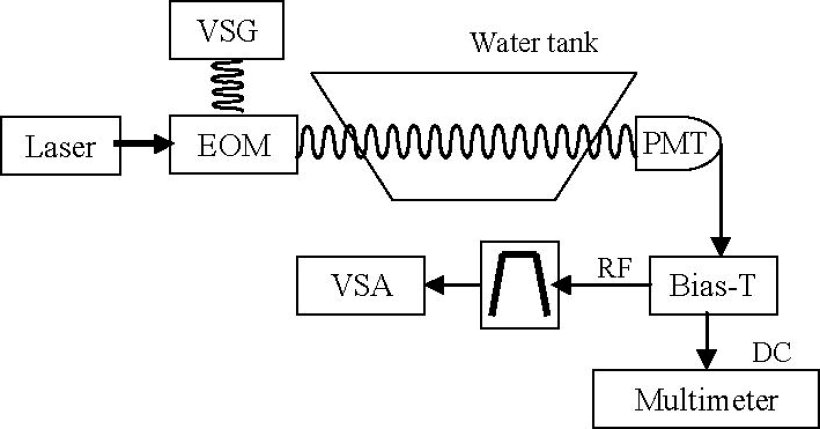
\includegraphics[width=0.8\textwidth]{coherent-source.jpg}
  \caption{Coherent Modulation using electro-optic modulator  \cite{cochenour_mullen_laux_2007}}
  \label{fig:boat1}
\end{figure}

\subsection{Channel Coding Schemes}
Error coding schemes can help mitigate the effect of underwater attenuation. Redundant bits are introduced into the transmitted bit sequence so that the receiver can correct a limited number of errors in the received message. This is known as \ac{FEC}.

It would be best to use convolutional codes if possible, as they can provide much higher \ac{BER} performance under harsh environments.

\subsubsection{Block Codes}
These codes add extra bits to each block, known as parity bits. These carry no extra information. They are simple to implement but are not as good as convolutional codes especially in turbid water or multiple scatters. Examples are \ac{RS} codes.

\subsubsection{Convolutional Codes}
Each code word depends on the message block but also a number of previous message blocks. This requires sequential logic circuits to implement and is thus harder to implement. They do however provide much higher performance. Examples are \ac{LDPC} and Turbo codes.

\section{System Aims}
The aim of the system that is being built at \ac{KAUST} is to provide a high speed point to point \ac{UOWC} link using lasers. The initial system will be static, but a sophisticated tracking system is being developed to ensure the lasers stay aligned with each other.

\subsection{Current System}

\subsubsection{Hardware}
The current system at \ac{KAUST} is built using a Nichia Green laser (NDG7K75T) as the transmitter, and a Thorlabs DET10A2 Si Biased Detector for the receiver.

The transmitter is connected via a Bias Tee to the UART TX line of a Raspberry Pi.

The receiver is connected via an amplifier and comparator, to the RX UART line of the Raspberry Pi.

This is duplicated on either side of the system, so that a full duplex system is realized.

\subsubsection{Software}
pppd is used to create an OOK link which is bridged to the Ethernet or WiFi interfaces.

\subsection{System Issues}
The main limitations of the system are as follows:

\subsubsection{Poor performance}
The current system is limited to a transmission rate of about 1 Mb/s. The use of the UART is the main limitation in terms of system performance. The baud rate cannot be pushed very high. In terms of interfaces, the Raspberry Pi has SPI, I2C and UART connections. None of these are suitable for a system targeting gigabit performance.

A system requires higher speed interfaces, such as gigabit Ethernet, \ac{SFP}, \ac{PCIe} or \ac{USB} 3.0 and above.

\subsubsection{\ac{AGC}}
Currently the system must be tuned depending on the range by manually adjusting the amplifier at the receiver. This system needs refining so that the adjustments can be made electronically and in real time.

In traditional \ac{AGC} the receiver starts each packet at maximum gain, which is then reduced as the preamble is received and the signal strength is measured.

Another approach would be to measure the signal strength out of band and adjust accordingly, although this will not adapt quickly to changes in the channel.

\subsubsection{Alignment}
The laser beam is very narrow. It is very difficult to align the two ends to ensure consistent system performance. Both sides must track the other in order to adjust their beams accordingly.

Beam alignment can be done in-band or out-of-band. In out-of-band, a different control mechanism is used to localize and track each station. There are two that are being thought about at the moment, the first being acoustic (which has been done previously) and the second using cameras to visually track the laser beam.

An in-band system would use the laser link itself and measure the \ac{SNR} or \ac{RSSI} values received whilst moving the laser slightly, to ensure the best angle is chosen.

If an in-band system is required, this must be factored in to the protocols used as time is required to utilize the lasers for measurements. This must be designed in from the outset and thus a system that understands beam forming and movable stations must be used. For example, an 802.11-based \ac{MAC} could be used, where the protocol allows for scanning time between nodes.

\section{Research Systems}
This section describes systems that have been developed in the lab but not commercialized.

\begin{table}[H]
\begin{tabular}{lllllll}
\textbf{Data Rate} & \textbf{Range} & \textbf{Spectrum} & \textbf{Modulation} & \textbf{RX Type} & \textbf{TX Type} & \textbf{Power} \\
1 Gbps             & 2m                  & 532nm                    & OOK       & APD                    & Laser                     & 10mW           \\
2.28 Mbps          & 50m                 & 470nm                    & DPIM                       & APD                    & LED                       & 10W            \\
1.2 Mbps           & 30m                 & 480nm                    & DPIM                       & APD                    & LED                       & 5W             \\
2.3 Gbps           & 7m                  & 520nm                    & OOK                        & APD                    & Laser                     & 12mW           \\
1.45 Gbps          & 4.8m                & 450nm                    & IM/DD OFDM                 & APD                    & Laser                     & 40mW           \\
4.8 Gbps           & 5.4m                & 450nm                    & 16-QAM-OFDM                & APD                    & Laser                     & 15mW           \\
1 Mbps             & 3m                  & 532nm                    & BPSK                       & PMT                    & Laser                     & 3W             \\
5 Mbps             & 3.6m                & 532nm                    & 32-QAM                     & PMT                    & Laser                     &                \\
1 Mbps             & 3.66m               & 405nm                    & OOK                        & PMT                    & Laser                     & 17mW           \\
161.35 Mbps        & 2m                  & 450nm                    & 16-QAM OFDM                & PIN                    & LED                       &               
\end{tabular}
\end{table}

\section{Current Optical Systems}
\subsection{\ac{UOWC}}
There currently exists two commercial \ac{UOWC} systems.

\subsubsection{Bluecomm \ac{UOWC}}
This is manufactured by Sonardyne, a UK based company. It utilizes high power \ac{LED}s with a range of products depending on application, from shallow water to deep water, and when there are artificial lights being used (for example on \ac{ROV}s). They claim a maximum transmission rate of 500 Mb/s but for very short distances; longer distances are limited to around 5 - 10 Mb/s.

\subsubsection{Anglerfish \ac{UOWC}}
The Anglerfish \ac{UOWC} provides full-duplex voice communication between two divers, again using \ac{LED}s. It is designed for the military, and is difficult to intercept because of the directionality and unknown modulation frequencies.

\subsection{Optical Wireless Communication}
As well as underwater systems, there are also terrestrial based commercial systems utilizing visible light.

\subsubsection{Li-Fi}
Li-Fi was coined by Professor Harald Haas. The aim is to run standard 802.11 protocols using visible light (using infrastructure already in place such as overhead bulbs), hence the similarity to Wi-Fi.

There are two companies involved with Li-Fi, but PureLifi is the only one with a system on the market. They offer the PL0300, an integrated device implementing an 802.11 compatible stack with a USB interface. They claim 86.4 Mb/s data rate.

See \url{https://purelifi.com/wp-content/uploads/2019/02/pureLiFi-PL0300-ASICDatasheet.pdf}

The other is Velmenni based in India.

\subsubsection{IrDA / IrLAN}
The Infrared Data Association provide a specification for gigabit transmissions using infrared light. IrLAN allows a unit to connect to a local area network. However, it has dropped out of use and there aren't really any available modules on the market anymore.

\subsection{Wired}
Wired interfaces designed for lasers may provide the exact requirements.

However, wired interfaces can really only provide point to point communications. They have no knowledge of multi-point setups. Due to the use of a very directional laser, however, this may not be an issue.

If in-band localization is required, a wired interface will not suffice.

\subsubsection{\ac{SFP}}

\url{https://www.snia.org/technology-communities/sff/specifications}

Breakout board

\url{https://sincsquared.com/sites/default/files/DataSheet_SS-SFP-SMA_0.pdf}

\url{https://osmocom.org/issues/3313}

\url{https://shop.trenz-electronic.de/en/TE0422-02-SFP-2-SMA-Adapter?path=Trenz_Electronic/Accessories/SFP/TE0422/REV02}

\ac{SFP} outputs differential signal so need a subtractor to change this to a single ended signal appropriate for the laser. I believe these are known as amplifiers. See \url{https://electronics.stackexchange.com/questions/341592/differential-to-single-ended}

\url{http://blog.svenbrauch.de/2017/02/19/homemade-10-mbits-laser-optical-ethernet-transceiver/}

\subsubsection{Koruza}
This is an implementation of \ac{SFP}-based optical transmissions using infra-red light.

KORUZA - \url{https://github.com/IRNAS/KORUZA}

KAUST already has some of these available to use. They claim up to 1 Gbit/s transfer rate. The nice thing about this project is that it is all open source, both the hardware and the software.

There are currently no available \ac{SFP} transceivers working at the visible light (350nm and 420nm).

\section{Conclusions}
This document has summarized a general background behind \ac{UOWC}, the current implementations and drawbacks, and improvements that can be made to the system.

\section{List of Acronyms}
\begin{acronym}
\acro{AGC}{Automatic Gain Control}
\acro{APD}{Avalanche Photodiode}
\acro{BER}{Bit Error Rate}
\acro{FEC}{Forward Error Correction}
\acro{FOV}{Field Of View}
\acro{IM/DD}{Intensity Modulation / Direct Detection}
\acro{ISI}{Inter-Symbol Interference}
\acro{I2C}{Inter-Integrated Circuit}
\acro{KAUST}{King Abdullah University of Science and Technology}
\acro{LDPC}{Low Density Parity Code}
\acro{LED}{Light Emitting Diode}
\acro{LOS}{Line Of Sight}
\acro{MAC}{Medium Access Controller}
\acro{NLOS}{Non Line Of Sight}
\acro{OFDM}{Orthogonal Frequency Division Multiplexing}
\acro{OOK}{On-Off Keying}
\acro{PCIe}{Peripheral Component Interconnect Express}
\acro{PIN}{P-I-N}
\acro{PMT}{Photo Multiplier Tube}
\acro{PPM}{Pulse Position Modulation}
\acro{PWM}{Pulse Width Modulation
\acro{P2P}{Peer to Peer}
\acro{RF}{Radio Frequency}
\acro{ROV}{Remotely Operated Vehicle}
\acro{RS}{Reed-Solomon}
\acro{RSSI}{Received Signal Strength Indicator}
\acro{SFP}{Small form-factor pluggable}
\acro{SNR}{Signal to Noise Ratio}
\acro{SPAD}{Single Photo Avalanche Diode}
\acro{SPI}{Serial Peripheral Interface}
\acro{UART}{Universal asynchronous receiver/transmitter}
\acro{UOWC}{Underwater Optical Wireless Communication}
\acro{USB}{Universal Serial Bus}
\end{acronym}


\bibliographystyle{plain}
\bibliography{research}

\end{document}\grid
